\chapter{Flexible Diffusion Modeling of Long Videos}
\label{ch:fdm}


\section{Introduction}\label{sec:intro}

Generative modeling of photo-realistic videos is at the frontier of what is possible with deep learning on currently-available hardware. Although related work has demonstrated modeling of short photo-realistic videos (e.g. 30 frames~\citep{weissenborn2019scaling}, 48 frames~\cite{clark2019adversarial} or 64 frames~\citep{ho2022video}), generating longer videos that are both coherent and photo-realistic remains an open challenge. A major difficulty is scaling: photorealistic image generative models~\citep{child2020very,dhariwal2021diffusion} are already close to the memory and processing limits of modern hardware.  A long video is at very least a concatenation of many photorealistic frames, implying resource requirements, long-range coherence notwithstanding, that scale with frame count. 

Attempting to model such long-range coherence makes the problem harder still, especially because in general every frame can have statistical dependencies on other frames arbitrarily far back in the video.
%Exhibiting such long-range coherence means that each frame should have statistical dependencies on other frames arbitrarily far back in the video, adding to the computational burden.
%
%A common workaround is to use a fixed-lag autoregressive model, which models a frame (or sequence of frames) conditioned only on the immediately preceding frames~\citep{yang2022diffusion}.
%
Unfortunately fixed-lag autoregressive models impose unrealistic conditional independence assumptions (the next frame being independent of frames further back in time than the autoregressive lag is problematic for generating videos with long-range coherence).  And while deep generative models based on recurrent neural networks (RNN) theoretically impose no such conditional independence assumptions, in practice they must be trained over short sequences~\cite{gruslys2016memory,saxena2021clockwork} or with truncated gradients~\citep{tallec2017unbiasing}.  Despite this, some RNN-based video generative models have demonstrated longer-range coherence, albeit without yet achieving convincing photorealistic video generation~\citep{saxena2021clockwork,babaeizadeh2021fitvid,denton2018stochastic,kim2019variational,babaeizadeh2017stochastic}.

%With no general limit on the number of frames that must be conditioned on to capture long-range dependencies, we argue against spending increasingly many resources on capturing dependencies on increasingly many frames.
In this work we embrace the fact that finite architectures will always impose conditional independences. The question we ask is: given an explicit limit $K$ on the number of video frames we can jointly model, how can we best allocate these frames to generate a video of length $N > K$? One option is to use the previously-described autoregressive model but, if $K=N/4$, we could instead follow \citet{ho2022video} by training two models: one which first samples every 4th frame in the video, and another which (in multiple stages) infills the remaining frames conditioned on those. To enable efficient exploration of the space of such sampling schemes, we propose a flexible architecture based on the diffusion model (DM) framework. This can sample any subset of video frames conditioned on observed values of any other subset of video frames. It therefore lets us explore a wide variety of previously untested sampling schemes while being easily repurposed for different generation tasks such as unconditional generation, video completion, and generation of videos of different lengths. Since our model can be flexibly applied to sample any frames given any others we call it a Flexible Diffusion Model, or FDM.

\paragraph{Contributions}
\textbf{(1)} At the highest level, we claim to have concurrently developed one of the first diffusion model (DM)-based video generative models~\cite{ho2022video,yang2022diffusion}. To do so we augment a previously-used DM image architecture~\cite{ho2020denoising,nichol2021improved} with a temporal attention mechanism including a novel relative (frame) position encoding network.  \textbf{(2)} The principal contribution of this paper, regardless, is a ``meta-learning'' training objective that encourages learning of a video generative model that can (a) be flexibly conditioned on any number of frames (up to computational resource constraints) at any time in the past and future and (b) be flexibly marginalized (to achieve this within computational resource constraints). \textbf{(3)} We demonstrate that our model can be used to efficiently explore the space of resource constrained video generation schemes, leading to improvements over prior work on several long-range video modeling tasks. \textbf{(4)} Finally, we release a new autonomous driving video dataset along with a new video generative model performance metric that captures semantics more directly than the visual quality and comparison metrics currently in widespread use.


\begin{figure}[t]
    \centering
    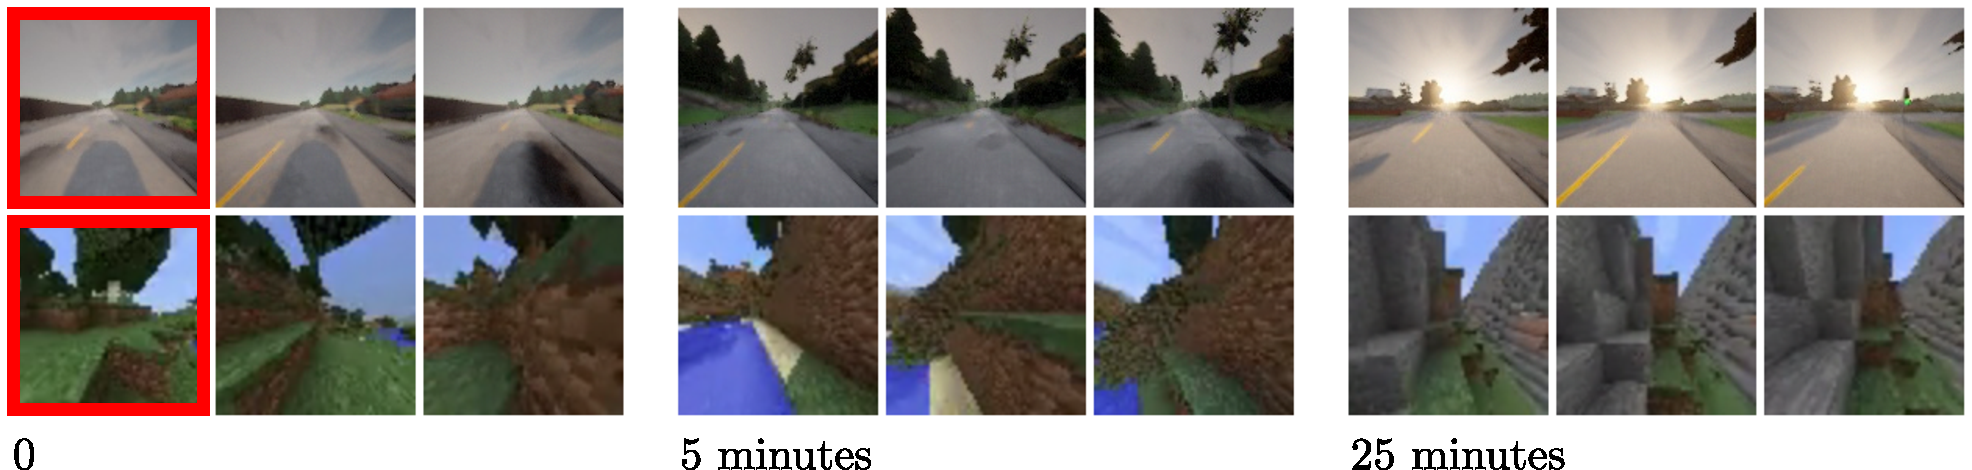
\includegraphics[width=\textwidth]{figs/fdm/fig1.pdf}
    \caption{A long video (25 minutes, or approximately 15\,000 frames) generated by FDM for each of CARLA Town01 and MineRL, conditioned on 500 and 250 prior frames respectively. We show blocks of frames from three points within each video, starting from the final observed frame on the left. Blocks are marked with the time elapsed since the last observation and frames within them are one second apart. We observe no degradation in sample quality even after $>15\,000$ frames.}
    \label{fig:1}
\end{figure}

% The net effect of this is that we can 1) unconditionally generate photorealistic, coherent video jointly, 2) we can conditionally generate video based on keyframes spread far into the past significantly expanding the Markov blanket of our artifact, and 3) we can conditionally generate video based on imagined futures, including imagined frames far in the future.  The latter has potentially profound implications for model-based reinforcement learning and planning, while the former leads to very significant improvements to video modeling performance on long-duration video completion benchmarks.

% There are alternatives to this autoregressive approach. One might follow \citet{ho2022video} and others \citep{} and learn both a joint distribution over a fixed number of ``key-frame'' subsampled in time from a long fixed length video as well as another, separate conditional video inpainting model which learns to jointly inpaint frames between such key-frames.  Such an architecture demonstrably encourages long-range coherence in generated videos while making efficient use of computational resource.  However, straightfoward application of such an artifact is most naturally suited to production of fixed length videos.  Less straightforward, but easy to imagine, are autoregressive generation methods based on sliding such an artifact forward in time so as to incrementally produce next keyframes one at a time after the first set and then inpaint to each new keyframe.  By virtue of dependence being captured at keyframe time resolution such an architecture and putative autoregressive mechanism might capture longer-range dependencies but still, effectively, would be constrained by autoregressive conditional independence limitations. 

% Our work breaks this conditional independence limitation to achieve extremely coherent, long-range video generation while elegantly addressing computational tractability.  At the highest level we claim to have concurrently developed one of the first denoising diffusion probabilistic model (DM)-based video generative models.  More granularly our DM-based video generative model, which we refer to as $\_\_\_\_\_\_$, has a number of sensible architectural innovations relative to DM-based image generative models \citep{} and the aforementioned DM-based video generative model \citep{ho2022video}.  Foremost amongst these are a relative (frame) position encoding network whose function and value is explained in detail later in the paper.  That aside, the principal contribution of this paper is an objective and ``meta-learning'' task schedule that encourages learning of a video generative model that can a) be flexibly conditioned on any number of frames (up to computational resource constraints) at any relative time in the past and future and b) be flexibly marginalized (to achieve this within computational resource constraints).  The net effect of this is that we can 1) unconditionally generate photorealistic, coherent video jointly, 2) we can conditionally generate video based on keyframes spread far into the past significantly expanding the Markov blanket of our artifact, and 3) we can conditionally generate video based on imagined futures, including imagined frames far in the future.  The latter has potentially profound implications for model-based reinforcement learning and planning, while the former leads to very significant improvements to video modeling performance on long-duration video completion benchmarks.


% In this work we show that through slight modification of the sampling procedure and network architecture in existing DM video models, we can train a single network with all of these capabilities. Specifically, unlike most prior work which trains on either consecutive or evenly spaced frames, we subsample video frames such that the training frames are no longer guaranteed to consecutive or evenly spaced, as shown in \cref{fig:mask-distribution-explanation}. We empirically demonstrate (\alert{do we?}) this results in a more flexibly trained network capable of generating frames conditioned on arbitrary subset of frames in a video. Second, prior work has shown improved performance can be obtained through the use of relative position embeddings in each temporal attention block. We show empirically (\alert{do we?}) that by replacing the lookup table mapping relative distance to vectors with a neural network, we achieve superior performance in terms of \alert{metric metric metric}. 

% Contributions:
% \begin{itemize}
%     \item We develop one of the first DM-based video generative models, concurrently with \citet{ho2022video,yang2022diffusion}.
%     \item Unlike this concurrent work, we jointly model sets of arbitrarily-spaced (i.e. not consecutive or evenly-spaced) frames, and innovate on the standard DM architecture for this use-case.
%     \item Using this flexible model, we perform a systematic comparison of various video sampling schemes.
%     \item We demonstrate that this leads to state-of-the-art performance on several long-range video modeling tasks as well as the ability to generate realistic videos leading to a specified end state.
%     \item We release a new autonomous driving video dataset along with a semantically meaningful performance metric.
% \end{itemize}




% \begin{figure}
% \begin{minipage}[t]{0.35\textwidth}
% \begin{algorithm}[H]
%     \centering
%     \caption{Sampling a video $\rvv$ given learned parameters $\theta$ and a sampling scheme $[(\mathcal{X}_s,\mathcal{Y}_s)]_{s=1}^S$.}%using learned parameters $\theta$ and a sampling scheme $[(\mathcal{X}_s,\mathcal{Y}_s)]_{s=1}^S$. }
%     \label{alg:sampling}
%     \footnotesize
%     \begin{algorithmic}[1]
% %        \State $\rvv \gets \texttt{zeros}(N, H, W, C)$
%         \For{$s \gets 1,\ldots,S$}
%             %\State $\rvy \gets [\text{$\rvv^i$ for $i$ in $\mathcal{Y}_s$}]$
%             % \For{$i \in 1:|\mathcal{Y}_s|$}
%             % \State $\rvy^i \gets \rvx^{\mathcal{Y}^i}$
%             % \EndFor
%             \State $\rvy \gets \rvx [\mathcal{Y}_s]$
%             \State $\rvx \sim  \texttt{DM}(\cdot; \rvy, \mathcal{X}_s, \mathcal{Y}_s, \theta)$
%             % \For{$i \in 1:|\mathcal{X}_s|$}
%             % \State $\rvv^{\mathcal{X}^i} \gets \rvx^i$
%             % \EndFor
%             \State $\rvv [\mathcal{X}_s] \gets \rvx$
%         \EndFor
%     \State \Return {$\rvv$}
%     \end{algorithmic}
% \end{algorithm}
% \end{minipage}
% \hfill
% \begin{minipage}[t]{0.64\textwidth}
% \begin{figure}[H]
%     \begin{subfigure}[t]{0.49\textwidth}
%         \centering
%         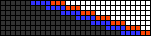
\includegraphics[width=\textwidth]{figs/fdm/unconditional-inference-modes/sample_vis_autoreg_T=30_sampling_3_out_of_7.png}
%         \caption{Autoregressive.} \label{fig:autoreg-vis}
%     \end{subfigure}
%     \begin{subfigure}[t]{0.49\textwidth}
%         \centering
%         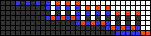
\includegraphics[width=\textwidth]{figs/fdm/unconditional-inference-modes/sample_vis_baby-cond-ho-et-al-for-vis_T=30_sampling_3_out_of_7.png}
%         \caption{Two temporal res.} \label{fig:google-vis}
%     \end{subfigure}
%     \begin{subfigure}[t]{0.49\textwidth}
%         \centering
%         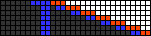
\includegraphics[width=\textwidth]{figs/fdm/unconditional-inference-modes/sample_vis_mixed-autoreg-independent_T=30_sampling_3_out_of_7.png}
%         \caption{Mixed (ours).} \label{fig:mixed-vis}
%     \end{subfigure}
%     \begin{subfigure}[t]{0.49\textwidth}
%         \centering
%         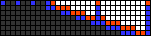
\includegraphics[width=\textwidth]{figs/fdm/unconditional-inference-modes/sample_vis_hierarchy-2_T=30_sampling_3_out_of_7.png}
%         \caption{Hierarchy-2 (ours).} \label{fig:hierarchy-vis}
%     \end{subfigure}%
% \end{figure}
% \end{minipage}
% \caption{\textbf{Left:} An algorithm for sampling a video $\rvv$ given learned parameters $\theta$ and a sampling scheme $[(\mathcal{X}_s,\mathcal{Y}_s)]_{s=1}^S$. \textbf{Right:} Visualisations of various sampling schemes for completing a video of length $N=30$ conditioned on the first ten frames, with access to at most $K=7$ frames at a time. Each stage $s$ of the sampling procedure is represented by one row in the figure, going from top to bottom. Within each subfigure, one column represents one frame of the video, from frame one on the left to frame 30 on the right. At each stage, the values of frames marked in red are sampled conditioned on the (observed or previously sampled) values of frames marked in blue. The gray frames are those which have been previously sampled but are ignored at a given stage. The white frames are yet to be sampled. After the final row, all video frames have been sampled in each case.
% }
% \label{fig:mask-distribution-explanation}
% \end{figure}

\section{Sampling long videos}

Our goal in this paper is to sample coherent photo-realistic videos $\rvv$ with thousands of frames (see \cref{fig:1}). 
%
%Our approach is to train a network which can, at test-time, be used to sample videos conditioned on specified values for any arbitrary subset of their frames, but for the sake of exposition we focus in this section on the case where only the start of the video is observed. 
%
To sample an arbitrarily long video with a generative model that can sample or condition on only a small number of frames at once, we must use a sequential procedure. The simplest example of this is an autoregressive scheme, an example of which is shown in \cref{fig:autoreg-vis} for a video completion task. 
%
In this example it takes seven stages to sample a complete video, in that we must run the generative model's sampling procedure seven times. 
%
At each stage three frames are sampled conditioned on the immediately preceding four frames. This scheme is appealing for its simplicity but imposes a strong assumption that, given the set of four frames that are conditioned on at a particular stage, all frames that come afterwards are conditionally independent of all frames that came before. This restriction can be partially ameliorated with the sampling scheme shown in \cref{fig:google-vis} where, in the first three stages, every second frame is sampled and then, in the remaining four stages, the remaining frames are infilled. One way to implement this would be to train two different models operating at the two different temporal resolutions. 
%
In the language of \citet{ho2022video}, who use a similar approach, sampling would be carried out in the first three stages by a ``frameskip-2'' model and, in the remaining stages, by a ``frameskip-1'' model. Both this approach and the autoregressive approach are examples of what we call \textit{sampling schemes}.
%
More generally, we characterize a sampling scheme as a sequence of tuples $[(\mathcal{X}_s, \mathcal{Y}_s)]_{s=1}^S$, each containing a vector $\mathcal{X}_s$ of indices of frames to sample and a vector $\mathcal{Y}_s$ of indices of frames to condition on for stages $s = 1,\ldots,S$. 

\Cref{alg:sampling} lays out how such a sampling scheme is used to sample a video. If the underlying generative model is trained specifically to model sequences of consecutive frames, or sequences of regularly-spaced frames, then the design space for sampling schemes compatible with these models is severely constrained. In this paper we take a  different approach.  We design and train a generative model to sample any arbitrarily-chosen subset of video frames conditioned on any other subset and train it using an entirely novel distribution of such tasks. In short, our model is trained to generate frames for any choice of $\mathcal{X}$ and $\mathcal{Y}$. The only constraint we impose on our sampling schemes is therefore a computational consideration that $|\mathcal{X}_s| + |\mathcal{Y}_s| \leq K$ for all $s$ but, to generate meaningful videos, any valid sampling scheme must also satisfy two more constraints: (1) all frames are sampled at at least one stage and (2) frames are never conditioned upon before they are sampled. %Our assumption about finite computational capacity imposes that the total number of frames sampled or conditioned on at any stage should always be below some constant $K$, i.e. $|\mathcal{X}_s| + |\mathcal{Y}_s| \leq K$ for any $s$.

\begin{algorithm}[t]
    \centering
    \caption{Sample a video $\rvv$ given a sampling scheme $[(\mathcal{X}_s,\mathcal{Y}_s)]_{s=1}^S$. For unconditional generation, the input $\rvv$ can be a tensor of zeros. For conditional generation, the observed input frames should contain their observed values.}
    \label{alg:sampling}
    \footnotesize
    \begin{algorithmic}[1]
    \Procedure{SampleVideo}{$\rvv$; $\theta$}
%        \State $\rvv \gets \texttt{zeros}(N, H, W, C)$
        \For{$s \gets 1,\ldots,S$}
            %\State $\rvy \gets [\text{$\rvv^i$ for $i$ in $\mathcal{Y}_s$}]$
            % \For{$i \in 1:|\mathcal{Y}_s|$}
            % \State $\rvy^i \gets \rvx^{\mathcal{Y}^i}$
            % \EndFor
            \State $\rvy \gets \rvv [\mathcal{Y}_s]$ \Comment{Gather frames indexed by $\mathcal{Y}_s$.}
            \State $\rvx \sim  \texttt{DM}(\cdot; \rvy, \mathcal{X}_s, \mathcal{Y}_s, \theta)$  \Comment{Sample $\rvx$ from the conditional DM.}
            % \For{$i \in 1:|\mathcal{X}_s|$}
            % \State $\rvv^{\mathcal{X}^i} \gets \rvx^i$
            % \EndFor
            \State $\rvv [\mathcal{X}_s] \gets \rvx$ \Comment{Modify frames indexed by $\mathcal{X}_s$ with their sampled values.}
        \EndFor
    \EndProcedure
    \State \Return {$\rvv$}
    \end{algorithmic}
\end{algorithm}


\begin{figure*}[t!]
    \centering
    \begin{subfigure}[t]{0.24\textwidth}
        \centering
        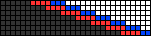
\includegraphics[width=\textwidth]{figs/fdm/unconditional-inference-modes/sample_vis_autoreg_T=30_sampling_3_out_of_7_red_blue_flipped.png}
        \caption{Autoregressive.} \label{fig:autoreg-vis}
    \end{subfigure}
    \begin{subfigure}[t]{0.24\textwidth}
        \centering
        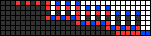
\includegraphics[width=\textwidth]{figs/fdm/unconditional-inference-modes/sample_vis_baby-cond-ho-et-al-for-vis_T=30_sampling_3_out_of_7_red_blue_flipped.png}
        \caption{Two temporal res.} \label{fig:google-vis}
    \end{subfigure}
    \begin{subfigure}[t]{0.24\textwidth}
        \centering
        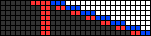
\includegraphics[width=\textwidth]{figs/fdm/unconditional-inference-modes/sample_vis_mixed-autoreg-independent_T=30_sampling_3_out_of_7_red_blue_flipped.png}
        \caption{Long-range (ours).} \label{fig:mixed-vis}
    \end{subfigure}
    \begin{subfigure}[t]{0.24\textwidth}
        \centering
        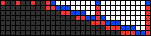
\includegraphics[width=\textwidth]{figs/fdm/unconditional-inference-modes/sample_vis_hierarchy-2_T=30_sampling_3_out_of_7_red_blue_flipped.png}
        \caption{Hierarchy-2 (ours).} \label{fig:hierarchy-vis}
    \end{subfigure}%
    \caption{Sampling schemes to complete a video of length $N=30$ conditioned on the first 10 frames, with access to at most $K=7$ frames at a time. Each stage $s$ of the sampling procedure is represented by one row in the figure, going from top to bottom. Within each subfigure, one column represents one frame of the video, from frame one on the left to frame 30 on the right. At each stage, the values of frames marked in blue are sampled conditioned on the (observed or previously sampled) values of frames marked in red; frames marked in gray are ignored; and frames marked in white are yet to be sampled. For every sampling scheme, all video frames have been sampled after the final row.
    }
\end{figure*}


Such a flexible generative model allows us to explore and use sampling schemes like those in \cref{fig:mixed-vis} and \cref{fig:hierarchy-vis}.  We find in our experiments that the best video sampling scheme is dataset dependent. Accordingly, we have developed methodology to optimize such sampling schemes in a dataset dependent way, leading to improved video quality as measured by the Fréchet Video Distance~\cite{unterthiner2018towards} among other metrics. We now review conditional DMs (\cref{sec:dm}), before discussing the FDM's architecture, the specific task distribution  used to train it, and the choice and optimization of sampling schemes in \cref{sec:architecture}.

\begin{figure*}[t]
    \centering
    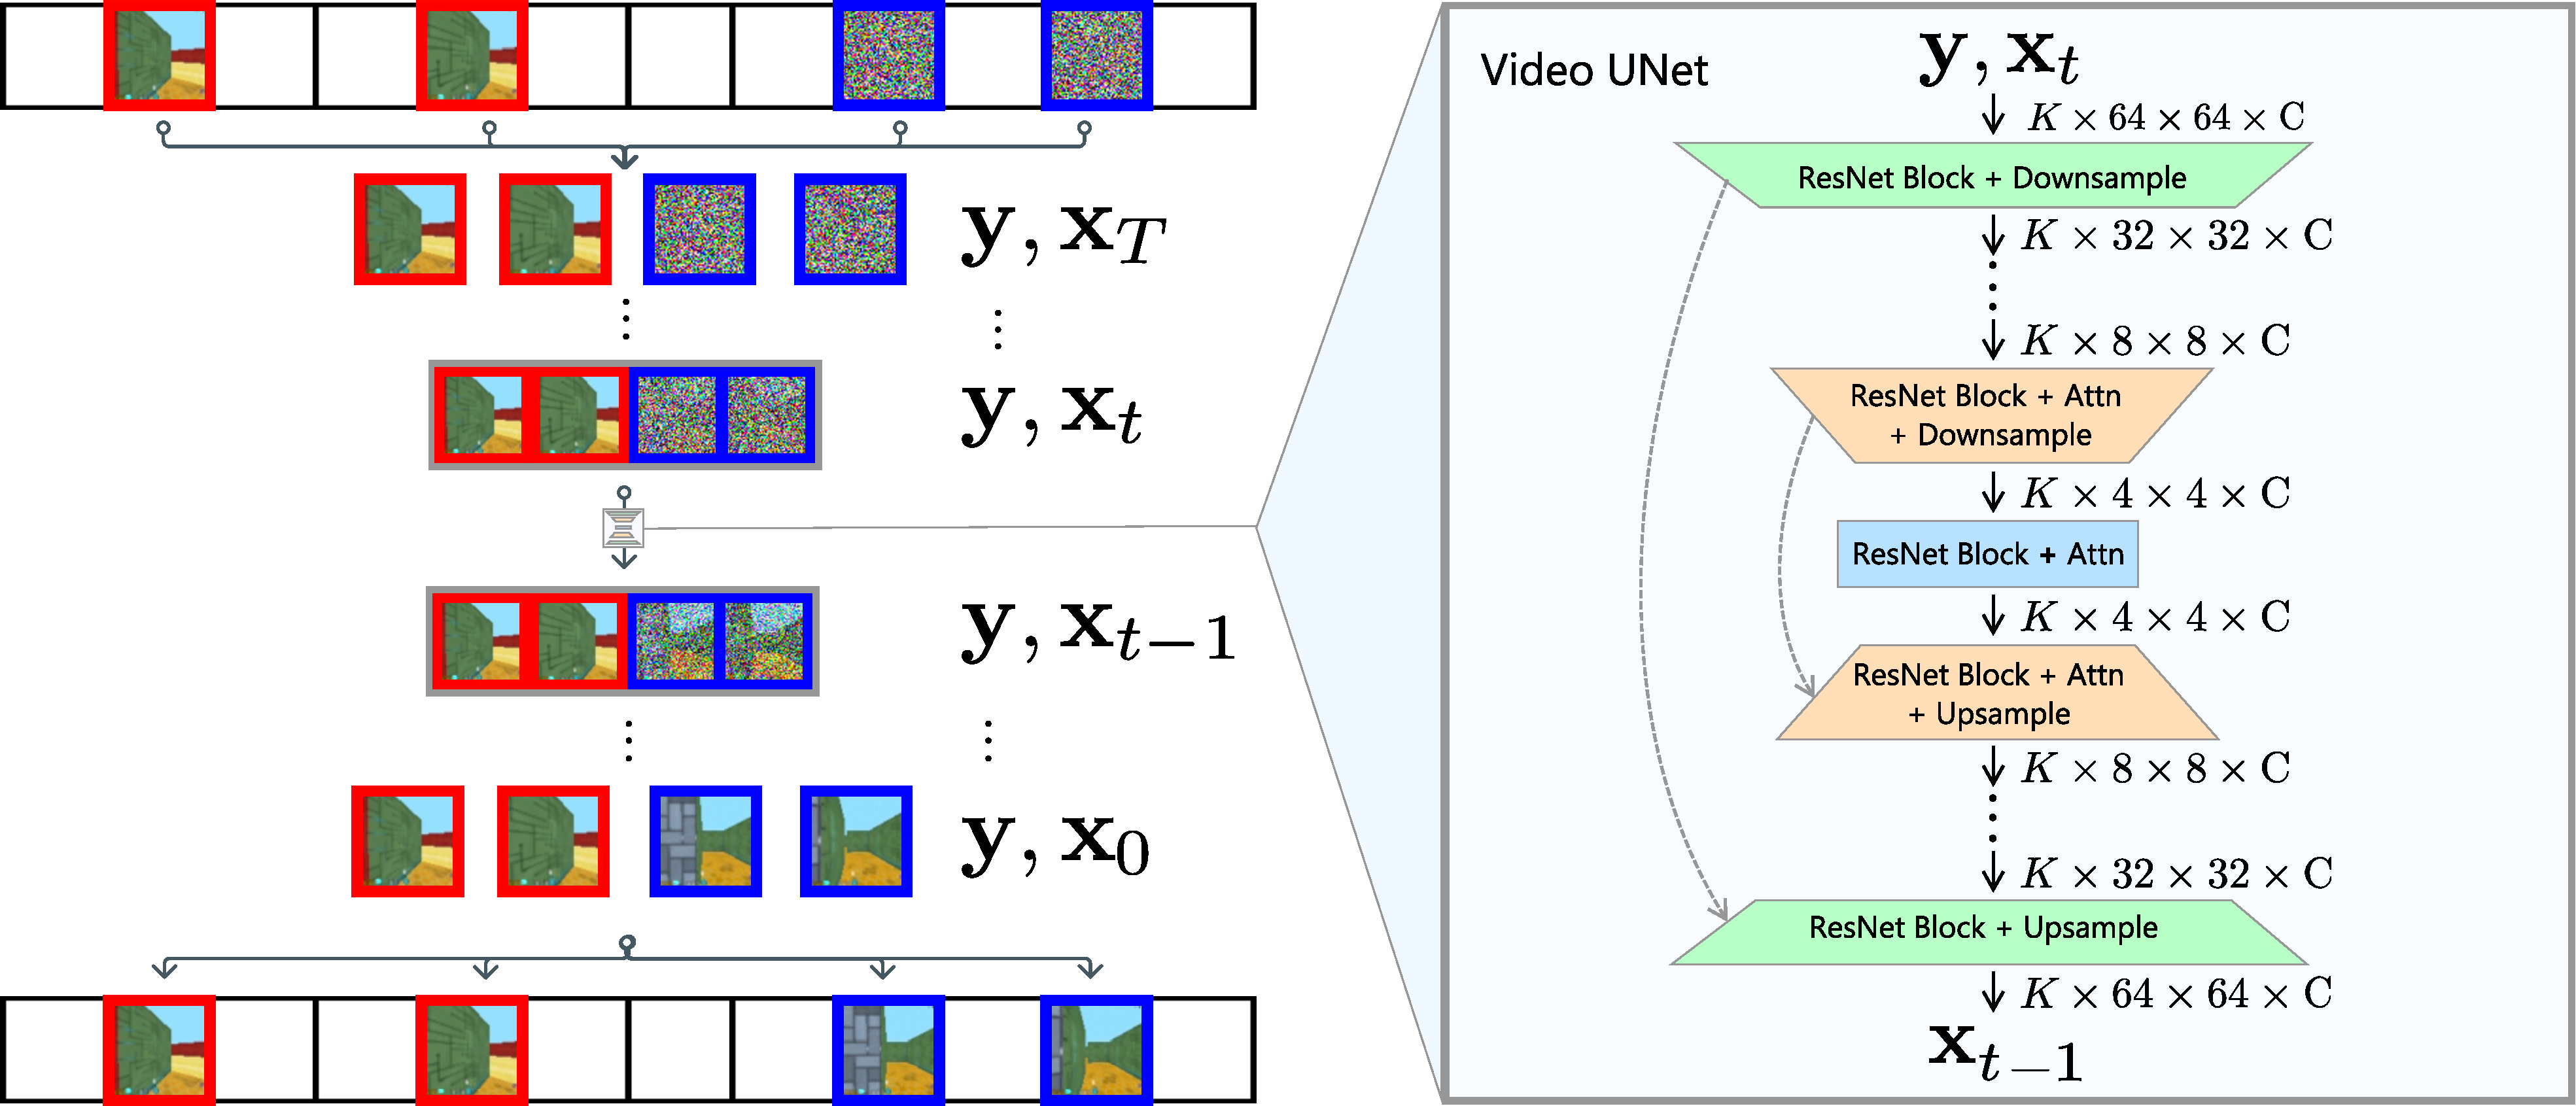
\includegraphics[width=0.88\textwidth]{figs/fdm/video-architecture-v8.pdf}
    \caption{\textbf{Left:} Our DM iteratively transforms Gaussian noise $\rvx_T$ to video frames $\rvx_0$ (shown with blue borders), conditioning on observed frames $\rvy$ (red borders) at every step. \textbf{Right:} The U-net architecture used within each DM step. It computes $\epsilon_\theta(\rvx_t, \rvy, t)$, with which the Gaussian transition $p_\theta(\rvx_{t-1}|\rvx_t)$ is parameterized.
    % On the left is the diffusion model which transforms Gaussian noise to video frames using the U-Net architecture (shown on the right) within each step of the diffusion process.  As described in \cref{sec:architecture}, we extend the U-net architecture used by \citet{nichol2021improved} for image sampling using temporal attention mechanisms, enhanced with neural relative position encodings, so that the embedding of each frame attend to other frames in the video sequence. Each upsampling/downsampling block consists of a residual neural network (ResNet) and skip connections shown in gray arrows. Spatial and temporal attention mechanism are applied to the inner blocks only (shown in orange), after the frames have been up/downsampled to $\le N \times 16 \times 16 \times C$. 
    }
    \label{fig:architecture}
\end{figure*}

% \section{A review of conditional denoising diffusion probabilistic models} \label{sec:dm}
% Denoising diffusion probabilistic models, or DMs~\citep{sohl2015deep,ho2020denoising,nichol2021improved,song2020score}, are a class of generative model for data $\rvx$, which throughout this paper will take the form of a 4-dimensional tensor representing multiple video frames. We will describe the conditional extension~\citep{tashiro2021csdi}, in which the modeled $\rvx$ is conditioned on observations $\rvy$. DMs simulate a diffusion process which transforms $\rvx$ to noise, and generate data by learning the probabilistic inverse of the diffusion process. The diffusion process happens over timesteps $0,\ldots,T$ such that $\rvx_0=\rvx$ is data without noise, $\rvx_1$ has a very small amount of noise added, and so on until $\rvx_T$ is almost independent of $\rvx_0$ and approximates a random sample from a unit Gaussian. In the diffusion process we consider, the distribution over $\rvx_t$ depends only on $\rvx_{t-1}$:
% \begin{equation} \label{eq:q-step}
%     q(\rvx_t | \rvx_{t-1}) = \gN(\rvx_t ; \sqrt{\alpha_t}  \rvx_{t-1} , (1-\alpha_t) \rmI ).
% \end{equation}

% Hyperparameters $\alpha_1,\ldots,\alpha_T$ are chosen to all be close to but slightly less than $1$ so that the amount of noise added at each step is small.
% The combination of this diffusion process and a data distribution $q(\rvx_0,\rvy)$ (recalling that $\rvx_0=\rvx$) defines the joint distribution
% \begin{equation} \label{eq:q-joint}
%     q(\rvx_{0:T}, \rvy) = q(\rvx_0, \rvy) \prod_{t=1}^T q(\rvx_t|\rvx_{t-1}).
% \end{equation}
% DMs work by ``inverting'' the diffusion process: given values of $\rvx_t$ and $\rvy$ a neural network is used to parameterize $p_\theta(\rvx_{t-1}|\rvx_t, \rvy)$, an approximation of $q(\rvx_{t-1}|\rvx_t,\rvy)$. This neural network lets us draw samples of $\rvx_0$ by first sampling $\rvx_T$ from a unit Gaussian (recall that the diffusion process was chosen so that $q(\rvx_T)$ is well approximated by a unit Gaussian), and then iteratively sampling $\rvx_{t-1} \sim p_\theta(\cdot|\rvx_t,\rvy)$ for $t=T,T-1,\ldots,1$. The joint distribution of sampled $\rvx_{0:T}$ given $\rvy$ is
% \begin{equation} \label{eq:p-joint}
%     p_\theta(\rvx_{0:T}|\rvy) = p(\rvx_{T}) \prod_{t=1}^T p_\theta(\rvx_{t-1}|\rvx_t, \rvy)
% \end{equation}
% where $p(\rvx_{T})$ is a unit Gaussian that does not depend on $\theta$. Training the conditional DM therefore involves fitting $p_\theta(\rvx_{t-1}|\rvx_t,\rvy)$ to approximate $q(\rvx_{t-1}|\rvx_t, \rvy)$ for all choices of $t$, $\rvx_t$, and $\rvy$.

% Several observations have been made in recent years which simplify the learning of $p_\theta(\rvx_{t-1}|\rvx_t,\rvy)$. \citet{sohl2015deep} showed that when $\alpha_t$ is close to 1, $p_\theta(\rvx_{t-1}|\rvx_t)$ is approximately Gaussian~\cite{sohl2015deep}. Furthermore, \citet{ho2020denoising} showed that this Gaussian's variance can be modeled well with a non-learned function of $t$, and that a good estimate of the Gaussian's mean can be obtained from a ``denoising model'' as follows. Given data $\rvx_0$ and unit Gaussian noise $\epsilon$, the denoising model (in the form of a neural network) is fed ``noisy'' data $\rvx_t := \sqrt{\tilde{\alpha}_t} \rvx_0 + \sqrt{1 - \tilde{\alpha}_t} \epsilon$ and trained to recover $\epsilon$ via a mean squared error loss. The parameters $\tilde{\alpha}_t := \prod_{i=1}^t \alpha_i$ are chosen to ensure that the marginal distribution of $\rvx_t$ given $\rvx_0$ is $q(\rvx_t|\rvx_0)$ as derived from \cref{eq:q-step}. Given a weighting function $\lambda(t)$, the denoising loss is
% \begin{equation} \label{eq:dm-loss}
%     \mathcal{L}(\theta) = \E_{q(\rvx_0, \rvy, \epsilon)} \left[ \sum_{t=1}^T \lambda(t) \lVert \epsilon - \epsilon_\theta(\rvx_t, \rvy, t) \rVert_2^2 \right] \quad \text{with} \quad \rvx_t = \sqrt{\tilde{\alpha}_t} \rvx_0 + \sqrt{1 - \tilde{\alpha}_t} \epsilon.
% \end{equation}
% The mean of $p_\theta(\rvx_{t-1}|\rvx_t,\rvy)$ is obtained from the denoising model's output $\epsilon_\theta(\rvx_t, \rvy, t)$ as ${\frac{1}{\alpha_t}\rvx_t - \frac{1-\alpha_t}{\sqrt{1-\tilde{\alpha}_t}}\epsilon_\theta(\rvx_t, \rvy, t)}$.
% If the weighting function $\lambda(t)$ is chosen appropriately, optimising \cref{eq:dm-loss} is equivalent to optimising a lower-bound on the data likelihood under $p_\theta$. In practice, simply setting $\lambda(t) := 1$ for all $t$ can produce more visually compelling results in the image domain~\citep{ho2020denoising}.


\section{Training procedure and architecture}\label{sec:method}

\paragraph{A note on notation with varying frame indices}
In our proposed method, as in \citet{tashiro2021csdi}, the shapes of $\rvx_0$ and $\rvy$ sampled from $q(\cdot)$ vary. This is because we want to train a model which can flexibly adapt to e.g. varying numbers of observed frames. To map \cref{eq:dm-loss} to this scenario, note that both $\rvx_0$ and $\rvy$ implicitly contain information about which frames in the video they represent (via the index vectors $\mathcal{X}$ and $\mathcal{Y}$ introduced in the previous section). This information is used inside the neural network $\epsilon_\theta(\rvx_t,\rvy, t)$ so that interactions between frames can be conditioned on the distance between them (as described in the following section) and also to ensure that the sampled noise vector $\epsilon$ has the same shape as $\rvx_0$.



\paragraph{Training task distribution}
Different choices of latent and observed indices $\mathcal{X}$ and $\mathcal{Y}$ can be regarded as defining different conditional generation tasks. In this sense, we aim to learn a model which can work well on any task (i.e. any choice of $\mathcal{X}$ and $\mathcal{Y}$) and so we randomly sample these vectors of indices during training. We do so with the distribution $u(\latindices,\obsindices)$ described in \cref{fig:training-distribution}. This provides a broad distribution covering many plausible test-time use cases while still providing sufficient structure to improve learning (see ablation in \cref{sec:experiments} and more details in \cref{app:training-task-dist-exp}). To cope with constrained computational resources, the distribution is designed such that $|\mathcal{X}|+|\mathcal{Y}|$ is upper-bounded by some pre-specified $K$. Sampling from $q(\rvx_0, \rvy)$ in \cref{eq:dm-loss} is then accomplished by randomly selecting both a full training video $\rvv$ and indices $\mathcal{X},\mathcal{Y}\sim u(\cdot,\cdot)$. We then extract the specified frames $\rvx = \rvv[\latindices]$ and $\rvy = \rvv[\obsindices]$ (where we use $\rvv[\latindices]$ to denote the concatenation of all frames in $\rvv$ with indices in $\latindices$ and and $\rvv[\obsindices]$ similarly).


% \Cref{alg:training} outlines our training procedure. This is similar to the standard dm training procedure~\cite{ho2020denoising} except that we use the conditional dm objective from \cref{eq:cond-dm-loss} and have an additional step where we sample the latent and observed indices $\mathcal{X},\mathcal{Y} \sim u(\cdot,\cdot)$. In our experiments, $N_\mathcal{X} + N_\mathcal{Y}$ is always bounded above by a small fraction of $N$, which allows us to train on videos with large $N$ without exceeding GPU memory limits. We now expand on our parameterisation of $u(\mathcal{X},\mathcal{Y})$.

% \paragraph{Latent and observe mask distribution}
% Key to our approach is the distribution $u(\mathcal{X},\mathcal{Y})$ over the indices of latent and observed frames used in training. Intuitively, to encourage good performance in practice, this should assign some probability to any $(\mathcal{X},\mathcal{Y})$ pair that is likely to be used. \todo{ablation with uniformly randomly sampled observes/latents?} Our parameterisation of $u$ is described in \cref{fig:mask-distribution-explanation}.

\begin{figure}
\begin{minipage}[t]{0.35\textwidth}
\begin{figure}[H]
%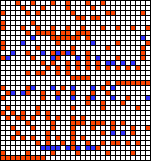
\includegraphics[width=\textwidth]{figs/fdm/more-example-masks.png}
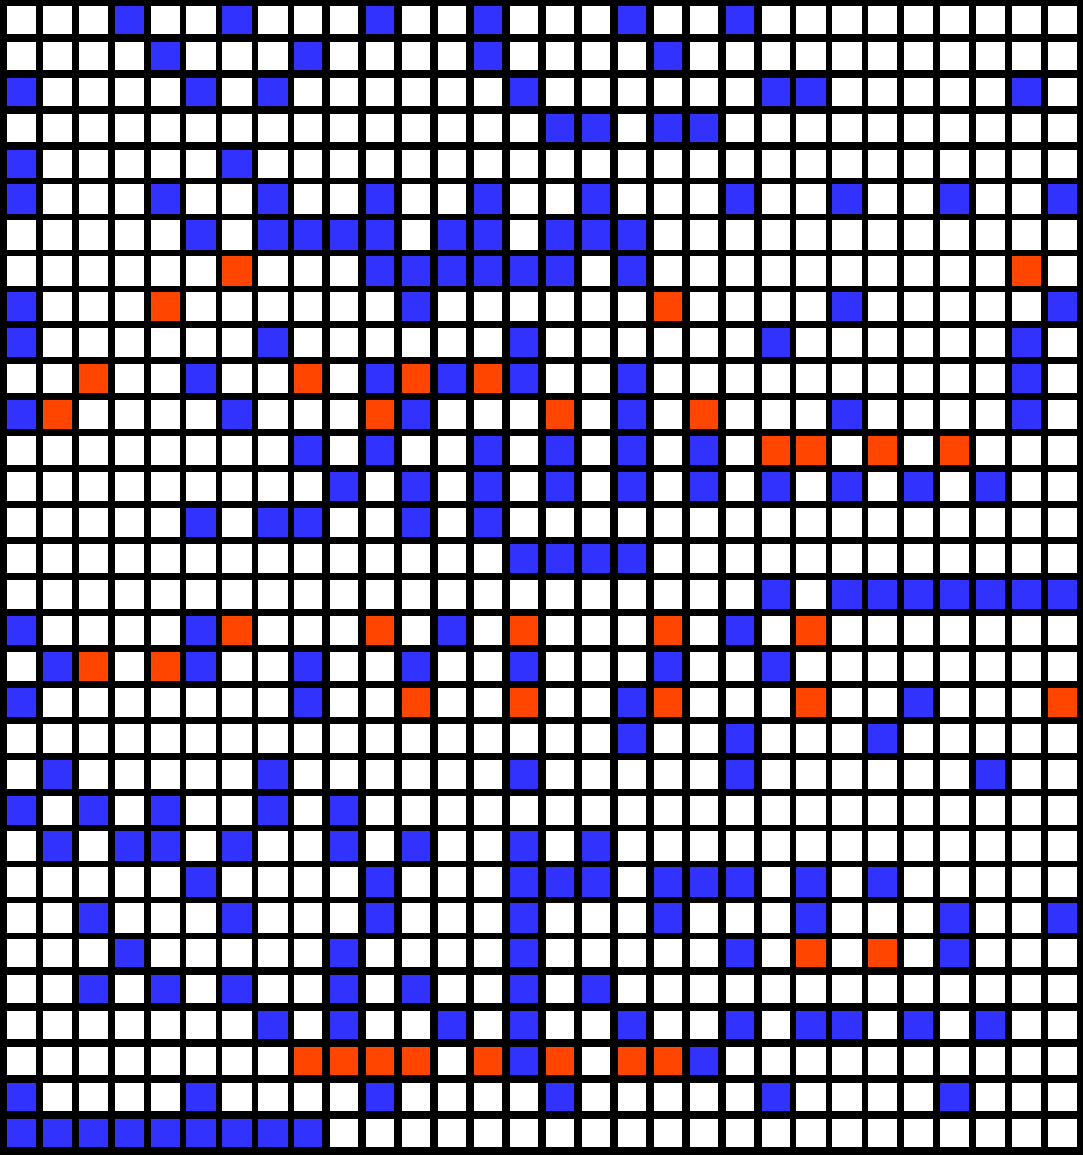
\includegraphics[width=\textwidth]{figs/fdm/training.pdf}
\end{figure}
\end{minipage}
\hfill
\begin{minipage}[t]{0.63\textwidth}
\begin{algorithm}[H]
    \caption{Sampling training tasks $\latindices,\obsindices\sim u(\cdot)$ given $N,K$.}\label{alg:mask-distribution}
    \label{alg:training-distribution}
    \footnotesize
    \begin{algorithmic}[1]
      \State $\latindices := \{\}$; $\obsindices := \{\}$
      \While{True}
        \State $n_\text{group} \sim \text{UniformDiscrete}(1, K)$ %\Comment{Sample number of frames in the group}
        \State $s_\text{group} \sim \text{LogUniform}(1, (N-1)/n_\text{group})$ %\Comment{Sample spacing between frames}
        \State $x_\text{group} \sim \text{Uniform}(0, N-(n_\text{group}-1)\cdot s_\text{group})$ %\Comment{Sample position of first frame in the group}
        \State $o_\text{group} \sim \text{Bernoulli}(0.5)$
        \State $\mathcal{G} := \{\lfloor x_\text{group} + s_\text{group} \cdot i \rfloor | i \in \{0,\ldots,n_\text{group}-1\} \} \setminus \latindices \setminus \obsindices$ \label{line:make-G}
        \If{$|\latindices| + |\obsindices| + |\mathcal{G}| > K$}
            \State \Return {$\texttt{set2vector}(\latindices),\texttt{set2vector}(\obsindices)$}
        \ElsIf{$|\latindices| = 0$ \textbf{or} $o_\text{group} = 0$} \label{line:obs-or-lat}
            \State $\latindices := \latindices \cup \mathcal{G}$
        \Else
            \State $\obsindices := \obsindices \cup \mathcal{G}$
        \EndIf
    \EndWhile
    \end{algorithmic}
\end{algorithm}
\end{minipage}
\caption{\textbf{Left:} Samples from $u(\mathcal{X},\mathcal{Y})$ with video length $N=30$ and limit $K=10$ on the number of sampled indices. Each row shows one sample and columns map to frames, with frame 1 on the left and frame $N$ on the right. Blue and red denote latent and observed frames respectively. All other frames are ignored and shown as white. \textbf{Right:} Pseudocode for drawing these samples. The while loop iterates over a series of regularly-spaced groups of latent variables. Each group is parameterized by: the number of indices in it, $n_\text{group}$; the spacing between indices in it, $s_\text{group}$; the position of the first frame in it, $x_\text{group}$, and an indicator variable for whether this group is observed, $o_\text{group}$ (which is ignored on line~\ref{line:obs-or-lat} if $\mathcal{X}$ is empty to ensure that the returned value of $\mathcal{X}$ is never empty). These quantities are sampled in a continuous space and then discretized to make a set of integer coordinates on line~\ref{line:make-G}. The process repeats until a group is sampled which, if added to $\latindices$ or $\obsindices$, will cause the number of frames to exceed $K$. That group is then discarded and $\mathcal{X}$ and $\mathcal{Y}$ are returned as vectors. The FDM's training objective forces it to work well for any $(\mathcal{X},\mathcal{Y})$ pair from this broad distribution.
}
\label{fig:training-distribution}
\end{figure}

\paragraph{Architecture}
\label{sec:architecture}
DM image models~\citep{ho2020denoising,nichol2021improved} typically use a U-net architecture~\cite{ronneberger2015u}. Its distinguishing feature is a series of spatial downsampling layers followed by a series of upsampling layers, and these are interspersed with convolutional res-net blocks~\cite{he2015deep} and spatial attention layers. Since we require an architecture which operates on 4-D video tensors rather than 3-D image tensors we add an extra \textit{frame} dimension to its input, output and hidden state, resulting in the architecture shown on the right of \cref{fig:architecture}. We create the input to this architecture as a concatenation $\rvx_t \oplus \rvy$, adding an extra input channel which is all ones for observed frames and all zeros for latent frames. For RGB video, the input shape is therefore $(K, \textit{image height}, \textit{image width}, 4)$. Since the output should have the same shape as $\rvx_t$ we only return outputs corresponding to the latent frames, giving output shape  $(|\latindices|, \textit{image height}, \textit{image width}, 3)$. We run all layers from the original model (including convolution, resizing, group normalization, and spatial attention) independently for each of the $K$ frames.
To allow communication between the frames, we add a temporal attention layer after each spatial attention layer, described in more detail in the appendix. 
%
The spatial attention layer allows each spatial location to attend to all other spatial locations \textit{within} the same frame, while the temporal attention layer allows each spatial location to attend to the same spatial location across all \textit{other} frames.
%
This combination of a temporal attention layer with a spatial attention layer is sometimes referred to as \textit{factorized attention}~\citep{tashiro2021csdi,ho2022video}. We found that, when using this architecture in conjunction with our meta-learning approach, performance could be improved by using a novel form of relative position encoding~\cite{shaw2018self,wu2021rethinking}. This is included in our released source code but we leave its exposition to the supplementary material.

\paragraph{Training batch padding}
Although the size $|\latindices\oplus\obsindices|$ of index vectors sampled from our training distribution is bounded above by $K$, it can vary. To fit examples with various sizes of index vectors into the same batch, one option would be to pad them all to length $K$ with zeros and use masks so that the zeros cannot affect the loss. This, however, would waste computation on processing tensors of zeros.
%
We instead use this computation to obtain a lower-variance loss estimate by processing additional data with ``training batch padding''.
%
This means that, for training examples where $|\latindices\oplus\obsindices| < K$, we concatenate frames uniformly sampled from a second video to increase the length along the frame-dimension to $K$. Masks are applied to the temporal attention mechanisms so that frames from different videos cannot attend to eachother and the output for each is the same as that achieved by processing the videos in different batches.

\paragraph{Sampling schemes}
% The central benefit of FDM is that training it once makes it easy to try out a wide variety of sampling schemes. 
%Each individual sampling scheme is not carefully tuned. 
Before describing the sampling schemes we explore experimentally, we emphasize that the relative performance of each is dataset-dependent and there is no single best choice. A central benefit of FDM is that it can be used at test-time with different sampling schemes without retraining. Our simplest sampling scheme, \textbf{Autoreg}, samples ten consecutives frames at each stage conditioned on the previous ten frames. \textbf{Long-range} is similar to Autoreg but conditions on only the five most recent frames as well as five of the original 36 observed frames. \textbf{Hierarchy-2} uses a multi-level sampling procedure. In the first level, ten evenly spaced frames spanning the non-observed portion of the video are sampled (conditioned on ten observed frames). In the second level, groups of consecutive frames are sampled conditioned on the closest past and future frames until all frames have been sampled. \textbf{Hierarchy-3} adds an intermediate stage where several groups of variables with an intermediate spacing between them are sampled. We include adaptive hierarchy-2, abbreviated \textbf{Ad. hierarchy-2}, as a demonstration of a sampling scheme only possible with a model like FDM. It samples the same frames at each stage as Hierarchy-2 but selects which frames to condition on adaptively at test-time with a heuristic aimed at collecting the maximally diverse set of frames, as measured by the pairwise LPIPS distance~\cite{zhang2018unreasonable} between them.

\paragraph{Optimizing sampling schemes}
An appealing alternative to the heuristic sampling schemes described in the previous paragraph would be to find a sampling scheme that is, in some sense, optimal for a given model and video generation/completion task. While it is unclear how to tractably choose which frames should be sampled at each stage, we suggest that the frames to condition on at each stage can be chosen by greedily optimizing the diffusion model loss which, as mentioned in \cref{sec:dm}, is closely related to the data log-likelihood. Given a fixed sequence of frames to sample at each stage $[\latindices_s]_{s=1}^S$ we select $\obsindices_s$ for each $s$ to minimize \cref{eq:dm-loss}. This is estimated using a set of 100 training videos and by iterating over 10 evenly-spaced values of $t$ (which reduced variance relative to random sampling of $t$). See the appendix for further details. We create two optimized sampling schemes: one with the same latent indices as Autoreg, and one with the same latent indices as Hierarchy-2. We call the corresponding optimized schemes \textbf{Opt. autoreg} and \textbf{Opt. hierarchy-2}.


\begin{figure}
    \centering
    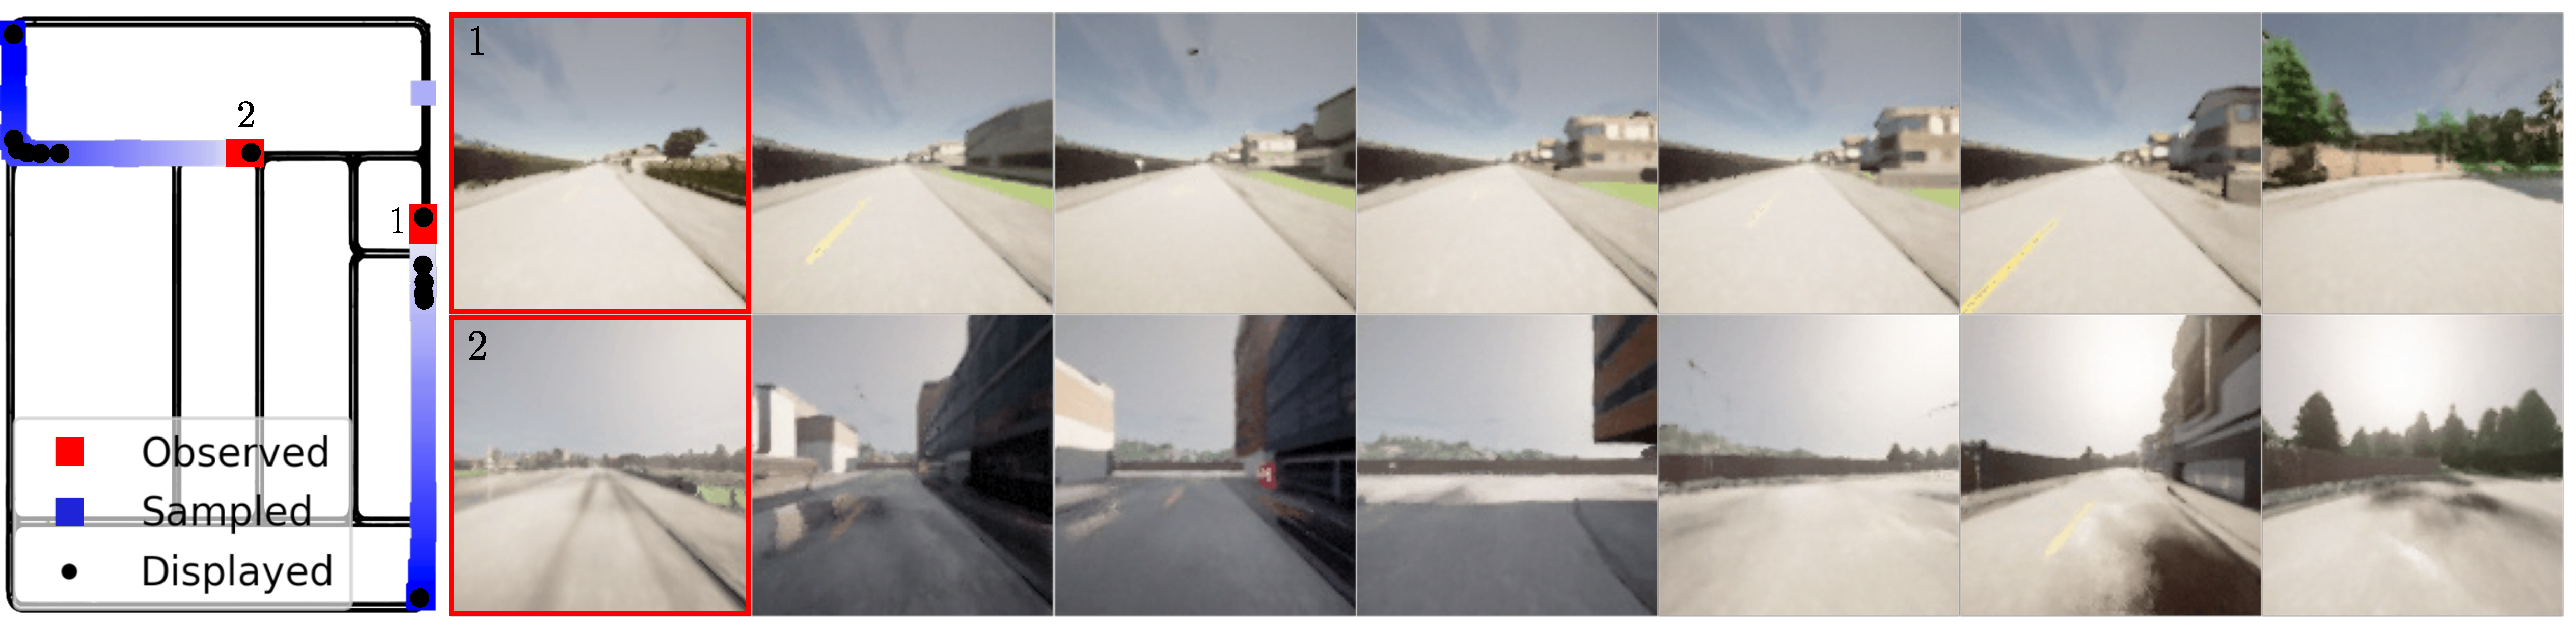
\includegraphics[width=1\textwidth]{figs/fdm/carla_map_7panel}
    \caption{\textbf{Left:} Map of the town featured in the CARLA Town01 dataset. We visualize two video completions by FDM by showing coordinates output by our regressor (discussed in \cref{sec:carla}) for each frame. Those corresponding to the initial 36 observed frames are shown in red and those for the 964 sampled frames are shown in blue. \textbf{Right:} For each completion, we show one of the initially observed frames followed by four of the sampled frames (at positions chosen to show the progression with respect to visible landmarks and marked by black dots on the map). The town's landmarks are usually sampled with high-fidelity, which is key to allowing the regressor  to produce a coherent trajectory on the left. However there are sometimes failures: a blue square near the top-right of the map shows where the video model ``jumped'' to a wrong location for a single frame.}
    \label{fig:carla}
\end{figure}


\section{CARLA Town01 Dataset}
\label{sec:carla}
In addition to our methodological contributions, we propose a new video-modeling dataset and benchmark which provides an interpretable measure of video completion quality. The dataset consists of videos of a car driving with a first-person view, produced using the CARLA autonomous driving simulator~\cite{dosovitskiy2017carla}.
%\footnote{Videos and data for training the regression model were supplied by InvertedAI using the CARLA autonomous vehicle simulator~\cite{dosovitskiy2017carla}.}
All 408 training and 100 test videos (of length 1000 frames and resolution $128\times128$) are produced within a single small town, CARLA's Town01. As such, when a sufficiently expressive video model is trained on this dataset it memorizes the layout of the town and videos sampled from the model will be recognisable as corresponding to routes travelled within the town. We train a regression model in the form of a neural network which maps with high accuracy from any single rendered frame to $(x,y)$ coordinates representing the car's position. Doing so allows us to plot the routes corresponding to sampled videos (see left of \cref{fig:carla}) and compute semantically-meaningful yet quantitative measures of the validity of these routes. Specifically, we compute histograms of speeds, where each speed is estimated by measuring the distance between the regressed locations for frames spaced ten apart (1 second at the dataset's frame rate). Sampled videos occasionally ``jump'' between disparate locations in the town, resulting in unrealistically large estimated speeds. To measure the frequency of these events for each method, we compute the percentage of our point-speed estimates that exceed a threshold of $10$m/s (the dataset was generated with a maximum simulated speed of $3$m/s). We report this metric as the outlier percentage (OP). After filtering out these outliers, we compute the Wasserstein distance (WD) between the resulting empirical distribution and that of the original dataset, giving a measure of how well generated videos match the speed of videos in the dataset. We release the CARLA Town 01 dataset along with code and our trained regression model to allow future comparisons.\footnote{\url{https://github.com/plai-group/flexible-video-diffusion-modeling}}

\section{Experiments} \label{sec:experiments}




We perform our main comparisons on the video completion task. In keeping with \citet{saxena2021clockwork}, we condition on the first 36 frames of each video and sample the remainder. We present results on three datasets: GQN-Mazes~\citep{eslami2018neural}, in which videos are 300 frames long; MineRL Navigate~\citep{guss2019minerl,saxena2021clockwork} (which we will from now on refer to as simply MineRL), in which videos are 500 frames long; and the CARLA Town01 dataset we release, for which videos are 1000 frames long. We train FDM in all cases with the maximum number of represented frames $K=20$. We host non-cherry-picked video samples (both conditional and unconditional) from FDM and all baselines online\footnote{\url{https://www.cs.ubc.ca/~wsgh/fdm}}.



\paragraph{Comparison of sampling schemes}
\begin{wrapfigure}[15]{r}{0.44\textwidth}
  \vspace{-.3cm}
  \begin{center}
    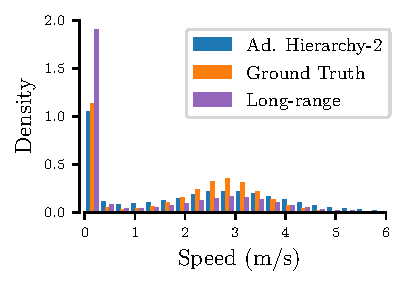
\includegraphics[width=0.44\textwidth]{figs/fdm/hist_new.pdf}
  \end{center}
  \caption{Speed distributions measured from sampled and ground-truth dataset videos.}
  \label{fig:hist}
\end{wrapfigure}
The relative performance of different sampling schemes varies significantly between datasets as shown in \cref{tab:fdm-results-completion}. We report Fréchet Video Distances (FVDs)~\cite{unterthiner2018towards}, a measure of how similar sampled completions are to the test set, on all datasets. In addition on GQN-Mazes we we report the accuracy metric~\cite{saxena2021clockwork}, which classifies videos based on which rooms are visited and measures how often a completion is given the same class as the corresponding test video. For CARLA Town01 we report the previously described percentage outliers (PO) and Wasserstein distance (WD) metrics. 

We can broadly consider the aforementioned sampling schemes as either being in the ``autoregressive'' family (Autoreg and Long-range) or in the ``hierarchical'' family (the remainder). Those in the hierarchical family achieve significantly better FVDs~\cite{unterthiner2018towards} on GQN-Mazes. Our samples in the appendix suggest that this is related to the autoregressive methods ``forgetting'' the colors of walls after looking away from them for a short time. In contrast, for MineRL the autoregressive methods tend to achieve the best FVDs. This may relate to the fact that trajectories in MineRL tend to travel in straight lines through procedurally-generated ``worlds''\cite{guss2019minerl,saxena2021clockwork}, limiting the number of long-range dependencies. 
Finally on CARLA Town01 we notice qualitatively different behaviours from our autoregressive and hierarchical sampling schemes. The hierarchical
sampling schemes have a tendency to occasionally lose coherence and ``jump'' 
to different locations in the town. This is reflected by higher outlier percentages (OP) in \cref{tab:fdm-results-completion}. On the other hand the autoregressive schemes often stay stationary for unrealistically long times at traffic lights. This is reflected in the histogram of speeds in \cref{fig:hist}, which has a larger peak around zero than the ground truth. The high variance of the sampling scheme's relative performance over different datasets points to a strength of our method, which need only be trained once and then used to explore a variety of sampling schemes. Furthermore, we point out that the best FVDs in \cref{tab:fdm-results-completion} on all datasets were obtained using sampling schemes that could not be implemented using models trained in prior work, or over evenly spaced frames.

\paragraph{Comparison with baselines}
The related work most relevant to ours is the concurrent work of \citet{ho2022video}, who model 64-frame videos using two trained DMs. The first is a ``frameskip-4'' model trained to generate every fourth frame and the second is a ``frameskip-1'' model trained on sequences of nine consecutive frames and used to ``fill in'' the gaps between frames generated in the first stage. To compare against this approach, which we denote \textbf{VDM}, we train both a ``frameskip-4'' and a ``frameskip-1'' model with architectures identical to our own.\footnote{The VDM is concurrent work and, at the time of writing, without a code-release. Since we intend this primarily as a comparison against the VDM sampling scheme we do not reimplement their exact architecture and note that there are other differences including their approach to imputation.} Since VDM requires two trained DMs, we train it for more GPU-hours than FDM despite the fact that FDM is meta-learning over a far broader task distribution. We also compare against \textbf{TATS}~\citep{ge2022long}, which embeds videos into a discrete latent space before modelling them with a transformers, and the clockwork VAE (\textbf{CWVAE})~\citep{saxena2021clockwork}, a VAE-based model specifically designed to maintain long-range dependencies within video.

Both the diffusion-based methods, FDM and VDM, achieve significantly higher FVD scores than TATS and CWVAE. This may point toward the utility of diffusion models in general for modeling images and video. \Cref{tab:fdm-results-completion} also makes clear the main benefit of FDM over VDM: although there is no sampling scheme for FDM which always outperforms VDM, there is at least one sampling scheme that outperforms it on each dataset. This speaks to the utility of learning a flexible model like FDM that allows different sampling schemes to be experimented with after training.

\begin{table*}
  \footnotesize
  \caption{Evaluation on video completion with various modes of our method along with several baselines from the literature. Error bars denote the standard error computed with 5 random seeds. Higher is better for the accuracy metric~\cite{saxena2021clockwork} and lower is better for all other metrics shown.}
  \label{tab:fdm-results-completion}
  \centering
  \begin{tabular}{llllllll}
    \toprule
    \multicolumn{1}{r}{} & & \multicolumn{2}{c}{GQN-Mazes}  & \multicolumn{1}{c}{MineRL}  & \multicolumn{3}{c}{CARLA Town01} \\
    \cmidrule(r){3-4} \cmidrule(r){5-5} \cmidrule(r){6-8}
    Model &  Sampling scheme        & FVD      & Accuracy  & FVD     &  FVD     & WD  & OP \\
    \midrule
    \multirow{1}{*}{CWVAE~\citep{saxena2021clockwork}}
    & CWVAE  & $837 \pm 8$      & $82.6 \pm 0.5$  & $1573 \pm 5$                 & $1161$          & $0.666$   & $44.4$        \\
    \midrule
    % \multirow{1}{*}{Autoreg.}& Autoreg.                 & $82.0$          & $6.28$        & $234$                 & $8.89$    & -          & -        \\
    % \midrule
    \multirow{1}{*}{TATS~\citep{ge2022long}}
    & TATS   & $163 \pm 2.6$  &  $77.0 \pm 0.8$  & $807 \pm 14$          & $329$          & $1.648$          & $42.4$ \\
    \midrule
    \multirow{1}{*}{VDM~\citep{ho2022video}}
    & VDM   & $66.7 \pm 1.5$  &  $77.8 \pm 0.5$  & $271 \pm 8.8$          & $169$          & $0.501$          & $16.9$ \\
    \midrule
    \multirow{5}{*}{FDM (ours)}
    &  Autoreg        & $86.4 \pm 5.2$          & $69.6 \pm 1.3$   & $281 \pm 10$          & $222$          & $0.579$      & $0.51$     \\
    &  Long-range           & $64.5\pm1.9$            & $77.0 \pm 1.4$   & $\mathbf{267 \pm 4.0}$     & $213$          & $0.653$      & $\mathbf{0.47}$     \\
    &  Hierarchy-2          & $\mathbf{53.1 \pm 1.1}$ & $82.8 \pm 0.7$   & $275 \pm 7.7$        & $120$     & $0.318$  &  $3.28$      \\
    &  Hierarchy-3          & $53.7 \pm 1.9$          & $\mathbf{83.8 \pm 1.1}$   & $311 \pm 6.8$        & $149$      & $0.363$    &  $4.53$  \\
    &  Ad. hierarchy-2      & $55.0 \pm 1.4$          & $83.2 \pm 1.3$   & $316 \pm 8.9$    & $\mathbf{117}$          & $\mathbf{0.311}$     & $3.44$    \\
    \bottomrule
  \end{tabular}
\end{table*}

\begin{table} %{r}{80mm}
  \small
  \caption{FVD scores for our sampling schemes with observed indices optimized offline as described in \cref{sec:method}.  We mark with an asterisk ($^*$) the eight numbers which improve on the corresponding non-optimized sampling schemes and highlight in bold those that are better than any in \cref{tab:fdm-results-completion}.}
  \vspace{2mm}
  \label{tab:fdm-optimized}
  \centering
  \begin{tabular}{lllllllll}
    \toprule
     & \multicolumn{2}{c}{GQN-Mazes}  & \multicolumn{1}{c}{MineRL}  & \multicolumn{3}{c}{CARLA Town01} \\
    \cmidrule(r){2-3} \cmidrule(r){4-4} \cmidrule(r){5-7}
    Sampling scheme       & FVD     & Accuracy    &    FVD & FVD & WD & OP \\
    \midrule
    Opt. autoreg        & $53.6 \pm 1.2^*$            & $80.2 \pm 1.2^*$            & $\mathbf{257 \pm 6.8}^*$    &   $146^*$ & $0.452^*$ & $0.65$   \\
    Opt. hierarchy-2   & $\mathbf{51.1 \pm 1.3}^*$    & $\mathbf{84.6 \pm 0.7}^*$   & $320 \pm 7.0$    &   $124$ & $0.349$ & $4.11^*$   \\
    \bottomrule
  \end{tabular}
\end{table}

\paragraph{Optimized sampling schemes}
% As mentioned in \cref{sec:method}, another advantage of FDM is that it makes possible a model- and dataset-specific optimization procedure to determine on which frames to condition. \Cref{tab:fdm-optimized} shows the results when this procedure is used to create sampling schemes for GQN-Mazes and MineRL. In the first row we show results where the latent frames are fixed to be those of the Autoreg sampling scheme, and in the second row the latent frames are fixed to match those of Hierarchy-2. In both cases the results in \cref{tab:fdm-results-completion} are improved upon, showing the utility of this optimization procedure.
As mentioned in \cref{sec:method}, another advantage of FDM is that it makes possible a model- and dataset-specific optimization procedure to determine on which frames to condition. \Cref{tab:fdm-optimized} shows the results when this procedure is used to create sampling schemes for different datasets. In the first row we show results where the latent frames are fixed to be those of the Autoreg sampling scheme, and in the second row the latent frames are fixed to match those of Hierarchy-2. On two of the three datasets the best results in \cref{tab:fdm-results-completion} are improved upon, showing the utility of this optimization procedure.

\paragraph{Comparison with training on a single task}
Training a network with our distribution over training tasks could be expected to lead to worse performance on a single task than training specifically for that task. To test whether this is the case, we train an ablation of FDM with training tasks exclusively of the type used in our Autoreg sampling scheme, i.e. ``predict ten consecutive frames given the previous ten.'' Tested with the Autoreg sampling scheme, it obtained an FVD of $82.0$ on GQN-Mazes and $234$ on MineRL. As expected given the specialization to a single task, this is better than when FDM is run with the Autoreg sampling scheme (obtaining FVDs of $86.4$ and $281$ respectively).

\paragraph{Ablation on training task distribution}
To test how important our proposed structured training distribution is to FDM's performance, we perform an ablation with a different task distribution that samples $\latindices$ and $\obsindices$ from uniform distributions instead of our proposed structured task distribution
%; and one which samples from an ablated variant of our task distribution where only one group of evenly-spaced frames is sampled (i.e. the while loop is ended after one iteration). 
We provide full details in the appendix, but report here that switching away form our structured training distribution made the FVD scores worse on all five tested sampling schemes on both GQN-Mazes and MineRL. The reduction in the average FVD was $31\%$ on GQN-Mazes and $52\%$ on MineRL. This implies that our structured training distribution has a significant positive effect.

\section{Related work}
Some related work creates conditional models by adapting the sampling procedure of an \textit{unconditional} DM~\citep{song2020score,kadkhodaie2020solving,mittal2021symbolic,ho2022video}. These approaches require approximations and the more direct approach that we use (explcitly training a conditional DM) was shown to have benefits by \citet{tashiro2021csdi}. We consider further comparison of these competing approaches to be outside the focus of this work, which is on modeling a small portion of video frames at a time, essentially performing marginalization in addition to conditioning.

There are a number of approaches in the literature which use VAEs rather than DMs for video modelling. \citet{babaeizadeh2017stochastic} use a VAE model which predicts frames autoregressively conditioned on a global time-invariant latent variable. A related approach by \citet{denton2018stochastic} also uses a VAE with convolutional LSTM architectures in both the encoder and decoder. Unlike \citet{babaeizadeh2017stochastic} the prior is learned and a different latent variable is sampled for each frame. \citet{babaeizadeh2021fitvid} use a VAE with one set of latent variables per frame and inter-frame dependencies tracked by a two-layer LSTM. Their architecture intentionally overfits to the training data, which when coupled with image augmentations techniques achieves SOTA on various video prediction tasks.  \citet{kim2019variational} use a variational RNN~\citep{chung2015recurrent} with a hierarchical latent space that includes binary indicator variables which specify how the video is divided into a series of subsequences. Both \citet{villegas2018hierarchical} and \citet{wichers2018learning} target long-term video prediction using a hierarchical variational LSTM architecture, wherein high-level features such as landmarks are predicted first, then decoded into low-level pixel space. The two approaches differ in that \citet{villegas2018hierarchical} requires ground truth landmark labels, while \cite{wichers2018learning} removes this dependence using an unsupervised adversarial approach. Fully GAN-based video models have also been proposed~\citep{aldausari2022video,clark2019adversarial} but generally suffer from ``low quality frames or low number of frames or both''~\citep{aldausari2022video}.

\section{Discussion}
%Our method is still slow to sample from. There are techniques to speed up sampling~\citep{salimans2022progressive,song2020denoising} but exploring them was outside the scope of this paper.

In this chapter we have defined and empirically explored a new method for generating photorealistic videos with long-range coherence that respects and efficiently uses fixed, finite computational resources.
Our approach outperforms prior work on long-duration video modeling as measured by quantitative and semantically meaningful metrics and opens up several avenues for future research.
For one, similar to using DMs for image generation, our method is slow to sample from (it takes approximately 16 minutes to generate a 300 frame video on a GPU).  Ideas for making sampling faster by decreasing the number of integration steps~\citep{salimans2022progressive,song2020denoising,xiao2022tackling} could be applied to our video model.  

On a different note, consider the datasets on which our artifact was trained.  In each there was a policy for generating the sequences of actions that causally led to the frame-to-frame changes in camera pose.  In MineRL the video was generated by agents that were trained to explore novel Minecraft worlds to find a goal block approximately 64 meters away~\cite{guss2019minerl}. The CARLA data was produced by a camera attached to an agent driven by a low level proportional–integral–derivative controller following waypoints laid down by a high level planner that was given new, random location goals to drive to intermittently. In both cases our video model had no access to either the policy or the specific actions taken by these agents and, so, in a formal sense, our models integrate or marginalize over actions drawn from the stochastic policy used to generate the videos in the first place.
%
Near-term future work could involve adding other modalities (e.g. audio) to FDM as well as explicitly adding actions and rewards, transforming our video generative model into a vision-based world model in the reinforcement learning sense~\citep{igl2018deep,kaiser2019model}. Furthermore, we point out that FDM trained on CARLA Town01 is in theory capable of creating 100-second videos conditioned on both the first and final frame. Doing so can be interpreted as running a ``visual'' controller which proposes a path between a current state and a specified goal.
%
Preliminary attempts to run in FDM in this way yielded inconsistent results but we believe that this could be a fruitful direction for further investigation.
